\documentclass[12pt]{article}

\usepackage[brazilian]{babel}
\usepackage{sbc-template}
\usepackage{times}
\usepackage{subfigure}



\usepackage[utf8]{inputenc}
\usepackage{xspace}

\usepackage[acronym,nowarn]{glossaries}
\newacronym{MPI}{MPI}{\textit{Message Passing Interface}}
\newcommand{\mpi}{\gls{MPI}\xspace}

\newacronym{openMP}{OpenMP}{\textit{Open Multi-Processing}}
    \newcommand{\openMP}{\gls{openMP}\xspace}

\newacronym{api}{API}{\textit{Application Programming Interface}}
    \newcommand{\api}{\gls{api}\xspace}
    \newcommand{\apis}{\glspl{api}\xspace}

\newacronym{cpu}{CPU}{\textit{Central Processing Unit}}
    \newcommand{\cpu}{\gls{cpu}\xspace}

    \newacronym{cpus}{CPUs}{\textit{Central Processing Units}}
    \newcommand{\cpus}{\gls{cpus}\xspace}

\newacronym{flops}{Flops}{\textit{Floating-point operations per second}}
    \newcommand{\flops}{\gls{flops}\xspace}

\newacronym{cnoc}{C-NoC}{\textit{Control NoC}}
    \newcommand{\cnoc}{\gls{cnoc}\xspace}

\newacronym{dnoc}{D-NoC}{\textit{Data NoC}}
    \newcommand{\dnoc}{\gls{dnoc}\xspace}

\newacronym{hpc}{HPC}{\textit{High Performance Computing}}
    \newcommand{\hpc}{\gls{hpc}\xspace}

\newacronym{mpsoc}{MPSoC}{\textit{Multiprocessor System-on-Chip}}
    \newcommand{\mpsoc}{\gls{mpsoc}\xspace}

\newacronym{noc}{NoC}{\textit{Network-on-Chip}}
    \newcommand{\noc}{\gls{noc}\xspace}
    \newcommand{\nocs}{\glspl{noc}\xspace}

\newacronym{pe}{PE}{\textit{Processing Element}}
    \newcommand{\pe}{\gls{pe}\xspace}
    \newcommand{\pes}{\glspl{pe}\xspace}

\newacronym{rm}{RM}{\textit{Resource Manager}}
    \newcommand{\rman}{\gls{rm}\xspace}
    \newcommand{\rmans}{\glspl{rm}\xspace}

\newacronym{smp}{SMP}{\textit{Symmetric Multiprocessing}}
    \newcommand{\smp}{\gls{smp}\xspace}

\newacronym{spmd}{SPMD}{\textit{Single Program, Multiple Data}}
    \newcommand{\spmd}{\gls{spmd}\xspace}

    \newacronym{simd}{SIMD}{\textit{Single Instruction, Multiple Data}}
    \newcommand{\simd}{\gls{simd}\xspace}

\newacronym{vliw}{VLIW}{\textit{Very Long Instruction Word}}
    \newcommand{\vliw}{\gls{vliw}\xspace}

\newacronym{gpu}{GPU}{\textit{Graphics Processing Unit}}
    \newcommand{\gpu}{\gls{gpu}\xspace}
    \newcommand{\gpus}{\glspl{gpu}\xspace}

\newacronym{rapl}{RAPL}{\textit{Running Average Power Limit}}
    \newcommand{\rapl}{\gls{rapl}\xspace}

\newacronym{lpddr}{LPDDR3}{\textit{Low Power Double Data Rate 3}}
    \newcommand{\lpddr}{\gls{lpddr}\xspace}

\newacronym{io}{E/S}{Entrada e Saída}
    \newcommand{\io}{\gls{io}\xspace}

\newacronym{ipc}{IPC}{\textit{Inter-Process Communication}}
   \newcommand{\ipc}{\gls{ipc}\xspace}

\newacronym{numa}{NUMA}{\textit{Non-Uniform Memory Access}}
	\newcommand{\numa}{\gls{numa}\xspace}

\newacronym{ccnuma}{CC-NUMA}{\textit{Cache-Coherent Non-Uniform Memory Access}}
\newcommand{\ccnuma}{\gls{ccnuma}\xspace}

\newacronym{ncnuma}{NC-NUMA}{\textit{No Cache Non-Uniform Memory Access}}
\newcommand{\ncnuma}{\gls{ncnuma}\xspace}

\newacronym{soc}{SoC}{\textit{System-on-Chip}}
\newcommand{\soc}{\gls{soc}\xspace}

\newacronym{cmp}{CMP}{\textit{Chip Multiprocessor}}
\newcommand{\cmp}{\gls{cmp}\xspace}

\newacronym{cmps}{CMPs}{\textit{Chip Multiprocessors}}
\newcommand{\cmps}{\gls{cmps}\xspace}


\newacronym{uma}{UMA}{\textit{Uniform Memory Access}}
    \newcommand{\uma}{\gls{uma}\xspace}

\newacronym{ram}{RAM}{\textit{Random-Access Memory}}
    \newcommand{\ram}{\gls{ram}\xspace}

\newacronym{pc}{PC}{\textit{Personal Computer}}
    \newcommand{\pc}{\gls{pc}\xspace}

\newacronym{opengl}{OpenGL}{\textit{Open Graphics Library}}
    \newcommand{\opengl}{\gls{opengl}\xspace}

\newacronym{cow}{COW}{\textit{Clusters of Workstations}}
    \newcommand{\cow}{\gls{cow}\xspace}


\newacronym{now}{NOW}{\textit{Network of Workstations}}
    \newcommand{\now}{\gls{now}\xspace}

    \newacronym{so}{SO}{\textit{Sistema Operacional}}
    \newcommand{\so}{\gls{so}\xspace}

    \newacronym{e/s}{E/S}{\textit{Entrada e Saída}}
    \newcommand{\es}{\gls{e/s}\xspace}

    \newacronym{kb}{KB}{\textit{Kilobyte}}
    \newcommand{\kb}{\gls{kb}\xspace}

    \newacronym{mb}{MB}{\textit{Megabyte}}
    \newcommand{\mb}{\gls{mb}\xspace}

    \newacronym{gb}{GB}{\textit{Gigabyte}}
    \newcommand{\gb}{\gls{gb}\xspace}

    \newacronym{posix}{POSIX}{\textit{Portable Operating System Interface}}
    \newcommand{\posix}{\gls{posix}\xspace}


\makeglossaries

\usepackage{todonotes}

\sloppy

\title{Execução Energeticamente Eficiente de Aplicações Estêncil com o Processador \textit{Manycore} MPPA-256}

\author{Emmanuel Podestá Jr.\inst{1}, Alyson D. Pereira\inst{1}, Rodrigo C. O. Rocha\inst{2},\\Márcio Castro\inst{1}, Luís F. W. Góes\inst{2}}

\address{
	Laboratório de Pesquisa em Sistemas Distribuídos (LaPeSD)\\
	Universidade Federal de Santa Catarina (UFSC) -- SC, Brasil
\nextinstitute{}
	Grupo de Computação Criativa e Paralela (CreaPar)\\
	Pontifícia Universidade Católica de Minas Gerais (PUC Minas) -- MG, Brasil
\email{emmanuel.podesta@grad.ufsc.br, alyson.pereira@posgrad.ufsc.br,}\\\vspace{-2em}\email{rcor@pucminas.br, marcio.castro@ufsc.br, lfwgoes@pucminas.br}}

\newcommand{\Fw}{\textit{Framework}\xspace}
\newcommand{\fw}{\textit{framework}\xspace}
\newcommand{\Fws}{\textit{Frameworks}\xspace}
\newcommand{\fws}{\textit{frameworks}\xspace}

\newcommand{\pskel}{PSkel\xspace}
\newcommand{\mppa}{MPPA-256\xspace}

\linespread{0.91}

\begin{document}

\maketitle

\begin{abstract}
In this paper is proposed an adaptation for the framework PSkel to the low-power
manycore processor \mppa. The framework simplifies iterative stencil
applications development to the \mppa, hiding implementation details from the
developer. The results on \mppa showed an energy consumption reduction on
iterative stencil applications up to 1.45x in comparison to the multicore
processor Intel Broadwell.
\end{abstract}

\begin{resumo}
Neste artigo é proposta uma adaptação do framework PSkel para o processador
\textit{manycore} de baixa potência \mppa. O \fw permite simplificar o
desenvolvimento de aplicações estêncil iterativas para o \mppa, escondendo do
desenvolvedor detalhes de implementação. Os resultados obtidos no \mppa
mostraram uma redução do consumo de energia de aplicações estêncil iterativas de
até 1.45x em comparação com um processador \textit{multicore} Intel Broadwell.
\end{resumo}

\section{Introdução}

Plataformas de Computação de Alto Desempenho (CAD) tem sido avaliadas quase que
exclusivamente pela suas capacidades de processamento. Contudo, o consumo
excessivo de energia é uma barreira para o aumento de desempenho de forma
escalável nestas plataformas. Por essa razão, o estudo de técnicas que melhorem
a eficiência energética em plataformas de CAD está se tornando muito importante.
Recentemente, uma nova classe de processadores \textit{manycore} de baixa
potência tais como o Sunway SW26010~\cite{sunway:2016} e o Kalray
\mppa~\cite{Castro-IA3:2013} foram desenvolvidos. Esses processadores possuem
centenas de núcleos de processamento capazes de lidar com paralelismo de dados e
tarefas com baixo consumo de energia.

Processadores \textit{manycore} de baixa potência (\textit{low-power manycore
    processors}) apresentam uma melhor eficiência energética em comparação com
processadores de propósito geral presentes
atualmente~\cite{Castro-IA3-JPDC:2014}, contudo as suas características
arquiteturais tornam o desenvolvimento de aplicações uma tarefa
desafiadora~\cite{Varghese14,Castro-PARCO:2016,Castro-SBAC-PAD:2014}.
% Geralmente, núcleos de processamento sem coerência de \textit{cache} são
% distribuídos em uma arquitetura organizada em \textit{clusters}, onde cada
% \textit{cluster} possui uma memória local (compartilhada somente entre os
% núcleos do \textit{cluster}). Dessa forma, a comunicação entre \textit{clusters}
% deve que ser efetuada através de uma \noc de maneira distribuída. Por essa
% razão, o tempo de comunicação pode variar entre os núcleos que estão se
% comunicando.
%
% Uma possível abordagem para facilitar o desenvolvimento de aplicações paralelas
% para processadores \textit{manycore} de baixa potência é através do uso de
% abstrações de mais alto nível fornecidas por padrões paralelos ou esqueletos
% algorítmicos~\cite{cole-skeleton:2004}. Esses padrões permitem que
% desenvolvedores foquem na construção de algoritmos, sem a preocupação com
% problemas de sincronização ou escalonamento de tarefas. Esses problemas são
% resolvidos de forma transparente pelo \fw do padrão adotado.

Existem diversos padrões paralelos para simplificar o desenvolvimento de
aplicações paralelas. Dentre eles (e.g., \textit{map}, \textit{reduce},
\textit{pipeline} e \textit{scan}), o padrão estêncil tem sido muito utilizado
em várias áreas importantes, como física quântica, previsão do tempo e
processamento de imagens~\cite{gonzalez06,holewinski12,lutz13}. No padrão
estêncil, para cada elemento de uma estrutura $n$-dimensional de entrada é
computado um novo valor para o respectivo elemento em uma estrutura
$n$-dimensional de saída, utilizando-se como base os valores dos elementos
vizinhos ao elemento de entrada. A quantidade de vizinhos e a computação a ser
realizada em cada elemento é definida por uma função (ou \textit{kernel})
estêncil. Em aplicações estêncil iterativas, os valores produzidos na estrutura
$n$-dimensional de saída em uma iteração $i$ são utilizados como entrada da
iteração $i+1$.

Alguns \fws foram propostos para o desenvolvimento de aplicações paralelas com
base no padrão estêncil, tais como SkelCL~\cite{steuwer11},
SkePU~\cite{enmyren10} e PSkel~\cite{pereira15}. Em especial, o \fw PSkel provê
uma abstração de alto nível para o desenvolvimento de aplicações estêncil em
ambientes heterogêneos compostos por processadores \textit{multicore} e
\textit{Graphical Processing Units} (GPUs). Todavia, nenhum desses \fws possui
suporte para processadores \textit{manycore} de baixo potência de energia
emergentes tais como o \mppa.

Portanto, nesse artigo é proposta uma adaptação completa do \fw \pskel para o
processador \mppa, a qual permite simplificar significativamente o
desenvolvimento de aplicações estêncil nesse processador. A adaptação permite
eliminar as dificuldades de desenvolvimento intrínsecas do processador, fazendo
com que as aplicações já implementadas em \pskel possam ser executadas no \mppa
sem a necessidade de nenhuma modificação em seus códigos. Os resultados obtidos
mostram que o \mppa apresenta uma melhor eficiência energética que um
processador Intel Broadwell com 10 núcleos físicos ao executar três aplicações
estêncil implementadas no \pskel.

O restante deste artigo está organizado da seguinte forma. A
Seção~\ref{sec:fundamentacao} apresenta os principais conceitos do processador
\textit{manycore} \mppa e do \fw \pskel. A Seção~\ref{sec:pskelMPPA} discute a
adaptação do \fw \pskel para fornecer suporte ao \mppa. Os resultados obtidos
com a adaptação do \fw \pskel para o \mppa são apresentados na
Seção~\ref{sec:resultados}. Por fim, a Seção~\ref{sec:conclusao} apresenta as
conclusões deste trabalho.

\section{Fundamentação Teórica}
\label{sec:fundamentacao}

\subsection{MPPA-256}
\label{subsec:mppa}

O \mppa é um processador \textit{manycore} desenvolvido pela empresa francesa
Kalray, o qual possui 256 núcleos de processamento de 400 MHz denominados \pes.
Além dos PEs, o processador possui 32 núcleos dedicados a gerência de recursos
denominados \textit{Resource Managers} (RMs). PEs e RMs são distribuídos
fisicamente no \textit{chip} em 16 \textit{clusters} e 4 subsistemas de
Entrada/Saída (E/S), contendo cada \textit{cluster} 16 PEs e 1 RM. Além dos
\textit{clusters}, o \mppa possui 4 subsistemas de E/S contendo, cada um, 4 RMs.
Toda a comunicação entre \textit{clusters} e/ou subsistemas de E/S é feita
através de uma \noc \textit{torus} 2D. A arquitetura do \mppa pode ser vista na
Figura~\ref{fig:config}a.

A finalidade principal dos PEs é executar \textit{threads} de usuário de forma
ininterrupta e não preemptível para realização de computação. PEs de um mesmo
\textit{cluster} compartilham uma memória de 2 MB, a qual é utilizada para
armazenar os dados a serem processados pelos PEs. Cada PE possui também uma
memória \textit{cache} associativa 2-\textit{way} de 32KB para dados e uma para
instruções. Porém, o processador não dispõe de coerência de \textit{caches}, o
que dificulta o desenvolvimento de aplicações para esse processador. Por outro
lado, a finalidade dos RMs é gerenciar E/S, controlar comunicações entre
\textit{clusters} e/ou subsistemas de E/S e realizar comunicação com uma memória
RAM. Na arquitetura utilizada neste artigo, um dos subsistemas de E/S está
conectado a uma memória externa \lpddr de 2 GB.

\begin{figure}[t]
	\centering
	\subfigure[fig:mppaOverall][\mppa.]{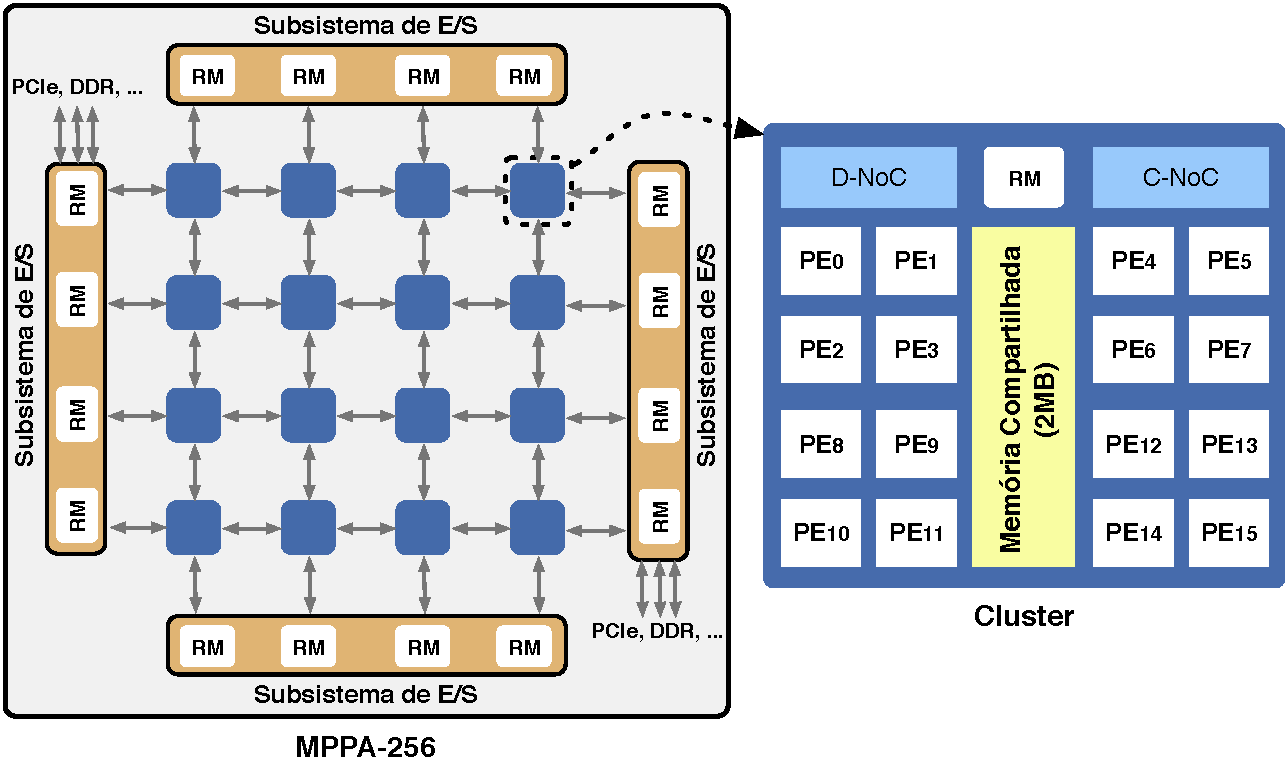
\includegraphics[width=0.43\textwidth]{figs/mppa-overview.pdf}}
	\qquad
	\subfigure[fig:stencil][O padrão estêncil.]{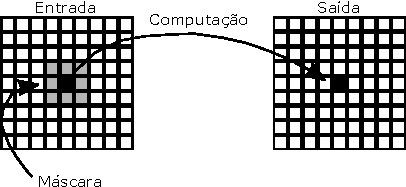
\includegraphics[width=0.4\textwidth]{figs/stencilComputation.pdf}}
    \caption{Visão geral do \mppa (esquerda) e uma ilustração do padrão estêncil oferecido pelo \pskel (direita).}
    \label{fig:config}
\end{figure}

Estudos anteriores mostraram que desenvolver aplicações paralelas otimizadas
para o \mppa é um grande desafio~\cite{Castro-IA3-JPDC:2014} devido a alguns
fatores importantes tais como: \textbf{(i) modelo de programação híbrido}:
\textit{threads} em um mesmo \textit{cluster} se comunicam através de uma
memória compartilhada local, porém a comunicação entre \textit{clusters} é feita
explicitamente via \noc, em um modelo de memória distribuída; \textbf{(ii)
comunicação}: é necessário a utilização de uma \api específica para a
comunicação via \noc, similar ao modelo clássico POSIX de baixo nível para \ipc;
\textbf{(iii) memória}: cada \textit{cluster} possui apenas 2 MB de memória
local de baixa latência, portanto aplicações reais precisam constantemente
realizar comunicações entre o subsistema de \io (conectado à memória \lpddr); e
\textbf{(iv) coerência de \textit{cache}}: cada \pe possui uma
memória \textit{cache} privada sem coerência com as \textit{caches} dos demais
\pes, sendo necessário o uso explícito de instruções do tipo \textit{flush} para
atualizar a \textit{cache} de um \pe em determinados casos.

\subsection{PSkel}
\label{subsec:pskel}

O \pskel é um \fw de programação em alto nível para o padrão estêncil, baseado
nos conceitos de esqueletos paralelos, que oferece suporte para execução
paralela em ambientes heterogêneos incluindo CPU e GPU.  Utilizando uma única
interface de programação escrita em C++, o usuário é responsável apenas por
definir o \textit{kernel} principal da computação estêncil, enquanto o \fw se
encarrega de gerar código executável para as diferentes plataformas paralelas,
realizando de maneira transparente todo o gerenciamento de memória e
transferência de dados entre dispositivos~\cite{pereira15}.

A Figura~\ref{fig:config}b ilustra o funcionamento da computação estêncil em
aplicações iterativas. Em cada iteração, uma máscara de vizinhança é utilizada
na matriz de entrada para determinar o valor de cada célula da matriz de saída.
Nesse exemplo, o valor de cada célula da matriz de saída é determinado em função
dos valores das células vizinhas em todas as direções. Esse processo é realizado
para todos os pontos da matriz de entrada, produzindo uma matriz saída da
computação estêncil. Ao final de uma iteração, a matriz de saída será
considerada como sendo a matriz de entrada da próxima iteração, gerando assim
uma nova matriz de saída ao final da próxima iteração.

\section{Adaptação do \fw \pskel para o \mppa}
\label{sec:pskelMPPA}

A adaptação do \fw \pskel para o processador \mppa proposta neste artigo segue
um modelo mestre/escravo. Um processo mestre é executado no subsistema de E/S
conectado à memória \lpddr de 2 GB, sendo responsável por alocar o
\texttt{Array} de entrada e por distribuir os dados entre os processos escravos.
Em cada \textit{cluster} é instanciado um único processo escravo que é
responsável por gerenciar a computação no seu \textit{cluster}. Devido às
limitações de memória dos \textit{clusters} (apenas 2~MB por \textit{cluster}),
o processo mestre deve subdividir o \texttt{Array} de entrada em blocos
denominados \textit{tiles} e, então, gerenciar as comunicações dos mesmos com os
processos escravos.

O processo mestre particiona o \texttt{Array} de entrada com dimensão $n$ em $b$
blocos, onde $b$ é o número de \textit{clusters} utilizados na computação.
Então, cada bloco é particionado em \textit{tiles} de tamanho fixo definidos
pelo usuário. Quando são feitas computações estêncil sobre o \textit{tile},
dependências de vizinhança, inerentes ao padrão paralelo do estêncil, precisam
ser consideradas durante o particionamento dos dados. Uma das principais
soluções para satisfazer essas dependências é via blocos sobrepostos, resultando
em dados redundantes e computação por
\textit{tile}~\cite{meng11,holewinski12,rocha17}. Essa técnica é muito
importante em \textit{manycores} de baixa potência como o \mppa, onde o
sobrecusto de comunicação pode ser elevado. O impacto dos custos de comunicação
será analisado posteriormente na Seção~\ref{sec:resultados}.


%\todo[inline]{A definição fala em um Array3D mas a figura mostra um Array2D. Não seria melhor falar de Array2D na definição?}
%Portanto, foi implementada uma técnica de \textit{tiling} trapezoidal no \fw \pskel. Para ilustrar e detalhar como essa técnica de \textit{tiling} pode ser aplicada na computação estêncil, utilizamos a definição a seguir. Seja $A$ um \texttt{Array3D}, com dimensões $\textrm{dim}(A)  =  (w,  h,  d)$, onde $w$,  $h$,  e  $d$ são, respectivamente, a largura, altura e profundidade. Utilizando \textit{tiles} de dimensões $(w^\prime, h^\prime, d^\prime)$ produz $\lceil\frac{w}{w^\prime}\rceil\lceil\frac{h}{h^\prime}\rceil\lceil\frac{d}{d^\prime}\rceil$ \textit{tiles} possíveis de $A$. Seja $A_{i,j,k}$ um \textit{tile}, onde
%$0\leq i < \lceil\frac{w}{ w^\prime}\rceil$,
%$0\leq j < \lceil\frac{h}{ h^\prime}\rceil$, e
%$0\leq k < \lceil\frac{d}{ d^\prime}\rceil$.
%$A_{i,j,k}$ possui \textit{offset} $(i w^\prime,j h^\prime,k d^\prime)$ relativo ao canto superior esquerdo de $A$ e $\textrm{dim}(A_{i,j,k}) = (
%\min\{w^\prime, w-i w^\prime\},
%\min\{h^\prime, h-j h^\prime\},
%\min\{d^\prime, d-k d^\prime\})$.
%O \textit{offset} é uma indexação de deslocamento necessário para acessar os elementos do \textit{tile} (Figura~\ref{fig:gputile}).

Portanto, foi implementada uma técnica de \textit{tiling} trapezoidal. Para
ilustrar e detalhar como essa técnica de \textit{tiling} pode ser aplicada na
computação estêncil, utilizamos a definição a seguir. Seja $A$ um
\texttt{Array2D}, com dimensões $\textrm{dim}(A)  =  (w,  h)$, onde $w$ e  $h$
são, respectivamente, a largura e a altura. Utilizando \textit{tiles} de
dimensões $(w^\prime, h^\prime)$ produz
$\lceil\frac{w}{w^\prime}\rceil\lceil\frac{h}{h^\prime}\rceil$ \textit{tiles}
possíveis de $A$. Seja $A_{i,j}$ um \textit{tile}, onde
$0\leq i < \lceil\frac{w}{ w^\prime}\rceil$ e
$0\leq j < \lceil\frac{h}{ h^\prime}\rceil$.
$A_{i,j}$ possui \textit{offset} $(i w^\prime,j h^\prime)$ relativo ao canto superior esquerdo de $A$ e $\textrm{dim}(A_{i,j}) = (
\min\{w^\prime, w-i w^\prime\},
\min\{h^\prime, h-j h^\prime\})$.
O \textit{offset} é uma indexação de deslocamento necessário para acessar os elementos do \textit{tile} (Figura~\ref{fig:gputile}).
Essa técnica pode ser facilmente estendida para mais dimensões.

\begin{figure}[t]
\centering
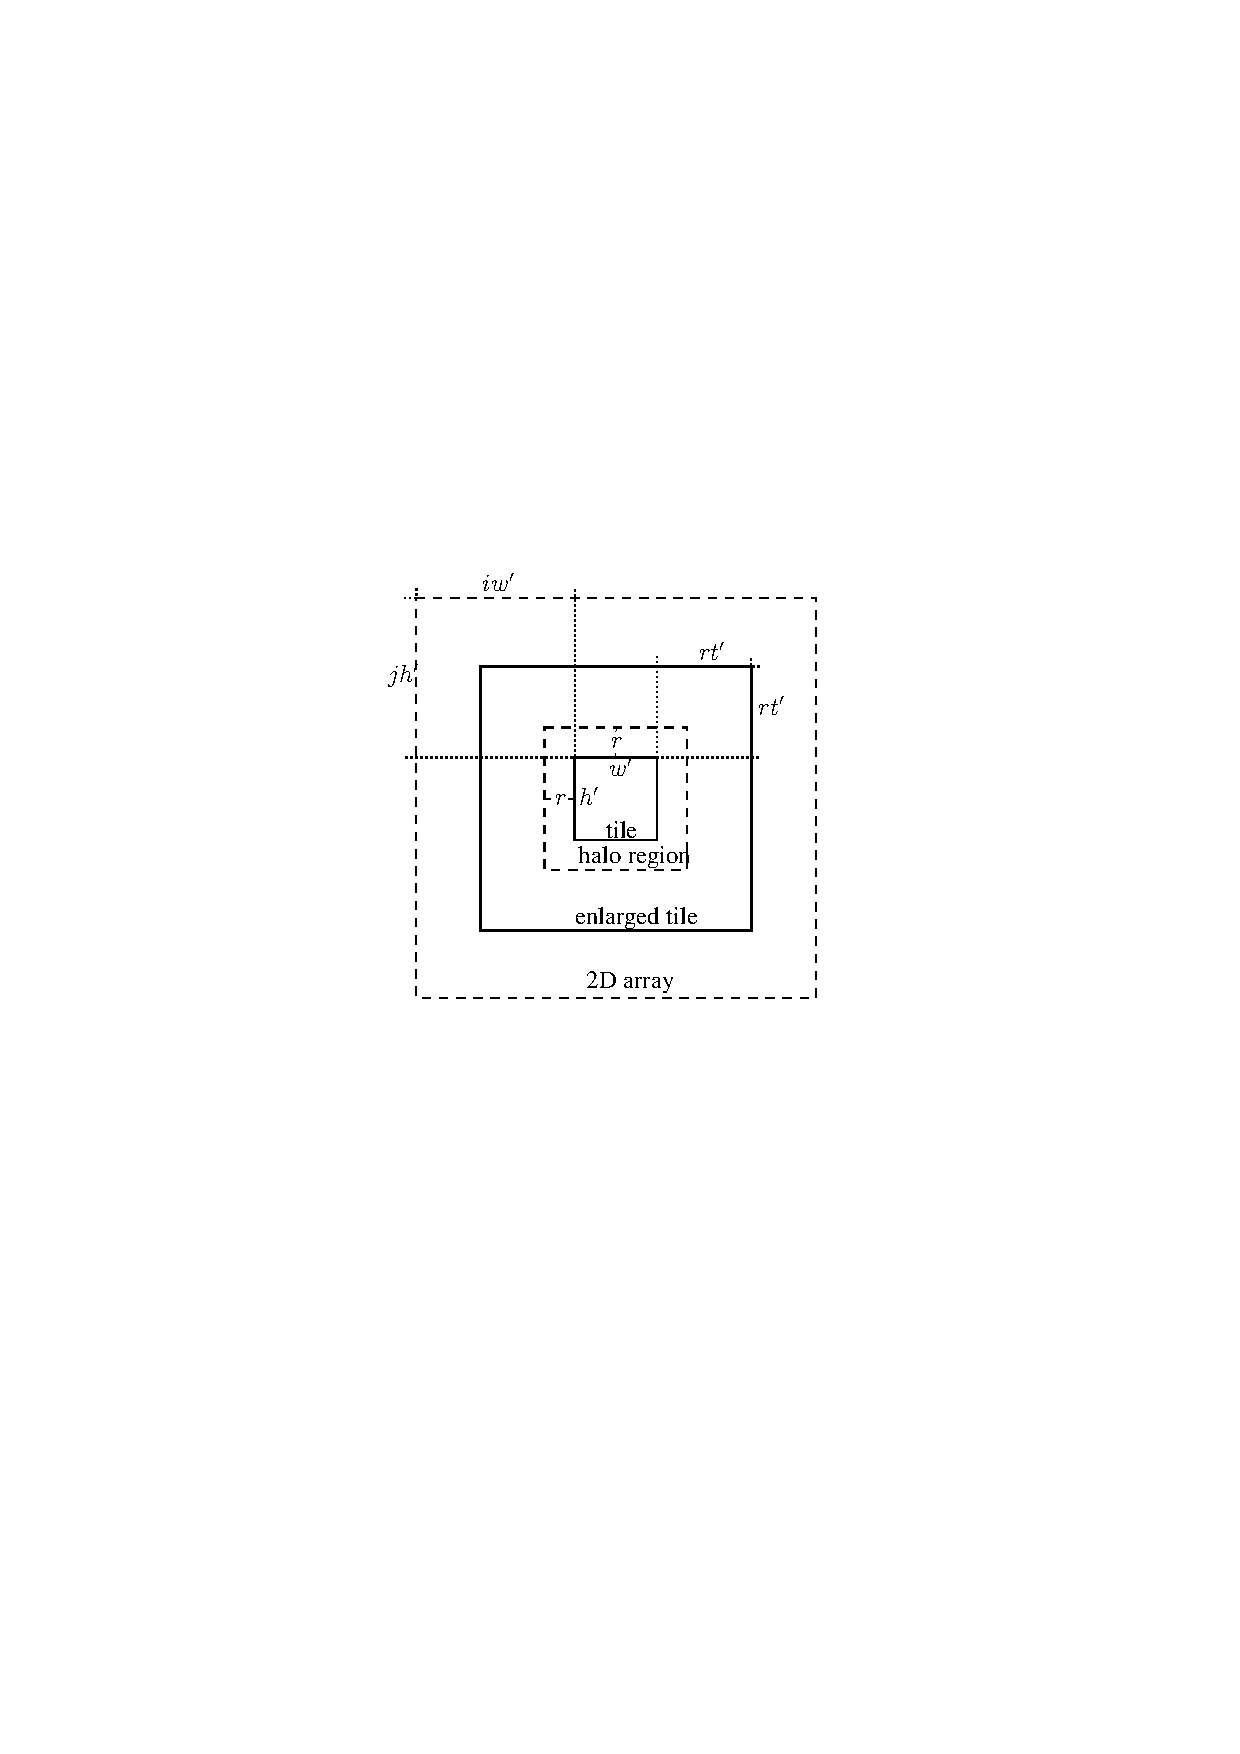
\includegraphics[width=0.3\columnwidth]{figs/tile.pdf}
\caption{ Diagrama do \textit{tiling} 2D. Um \textit{tile} lógico (linha interna sólida) é contido dentro do Array
    2D (linha externa pontilhada) com \textit{offsets} verticais e horizontais dado por $j  h^\prime$
    e $i  w^\prime$. Computar $t^\prime$ consecutivas iterações estêncil no \textit{tile} requer um aumento no
    \textit{tile} lógico com uma \textit{ghost zone} (área entre a linha interna sólida e a linha externa sólida), que é constituída
    de regiões \textit{halo} (área entre a linha interna sólida e a linha interna pontilhada).}
\label{fig:gputile}
%\vspace{-4em}
\end{figure}

Aplicar um estêncil em $A$ envolve aplicar a função de vizinhança (máscara)
contendo o deslocamento de cada vizinho de um dado elemento central. Por causa
da dependência entre vizinhos, para computar a função estêncil, de acordo com as
limitações necessárias pelos \textit{tiles}, se torna necessário obter valores
de \textit{tiles} adjacentes. Seja $r$ o \textit{range} da máscara de vizinhos,
i.e., $r$ é o deslocamento mais distante necessário para a vizinhança definida
pela máscara. A área de $r$ envolvendo a vizinhança é denominada região
\textit{halo}. Se a função estêncil é aplicada iterativamente sobre $A$, para
$t$ iterações, a dependência da vizinhança entre os \textit{tiles} limita o
número de iterações que podem ser computadas consecutivamente sem a necessidade
de realizar comunicações entre \textit{tiles}.

Além disso, devido à restrição da \api e \noc no \mppa, os dados armazenados em
cada \textit{tile} precisam ser contíguos para serem transferidos pela \noc. A
fim de se evitar cópias locais de dados, o que desperdiçaria memória e tempo de
processamento, utiliza-se o conceito de comunicação por \textit{strides}. Cada
\textit{stride} é uma parte contígua do \texttt{Array} original, sendo
determinado por deslocamentos (\textit{offsets}) especificados durante a
execução. Então, cada \textit{stride} é enviado para o \texttt{Array} de entrada
em um processo escravo na posição determinada de acordo com o tamanho dos
\textit{tiles} e do \texttt{Array} original. O método de \textit{strides}
possibilita a definição de algumas variáveis para o gerenciamento do
\texttt{Array}, sendo a mais importante os \textit{offsets} que serão
utilizados. A partir deles, o método irá efetuar a comunicação de maneira direta
para o\texttt{Array} destino. Como dito anteriormente, a utilização de
\textit{tiles} aumentados permite reduzir a quantidade de comunicações
necessárias entre os processos mestre e escravos. Fazendo o aumento dos
\textit{tiles} em uma dimensão temporal, os processos escravos podem executar
múltiplas iterações sem a necessidade de comunicação ou sincronização com o
processo mestre.

\begin{figure}[t]
	\centering
	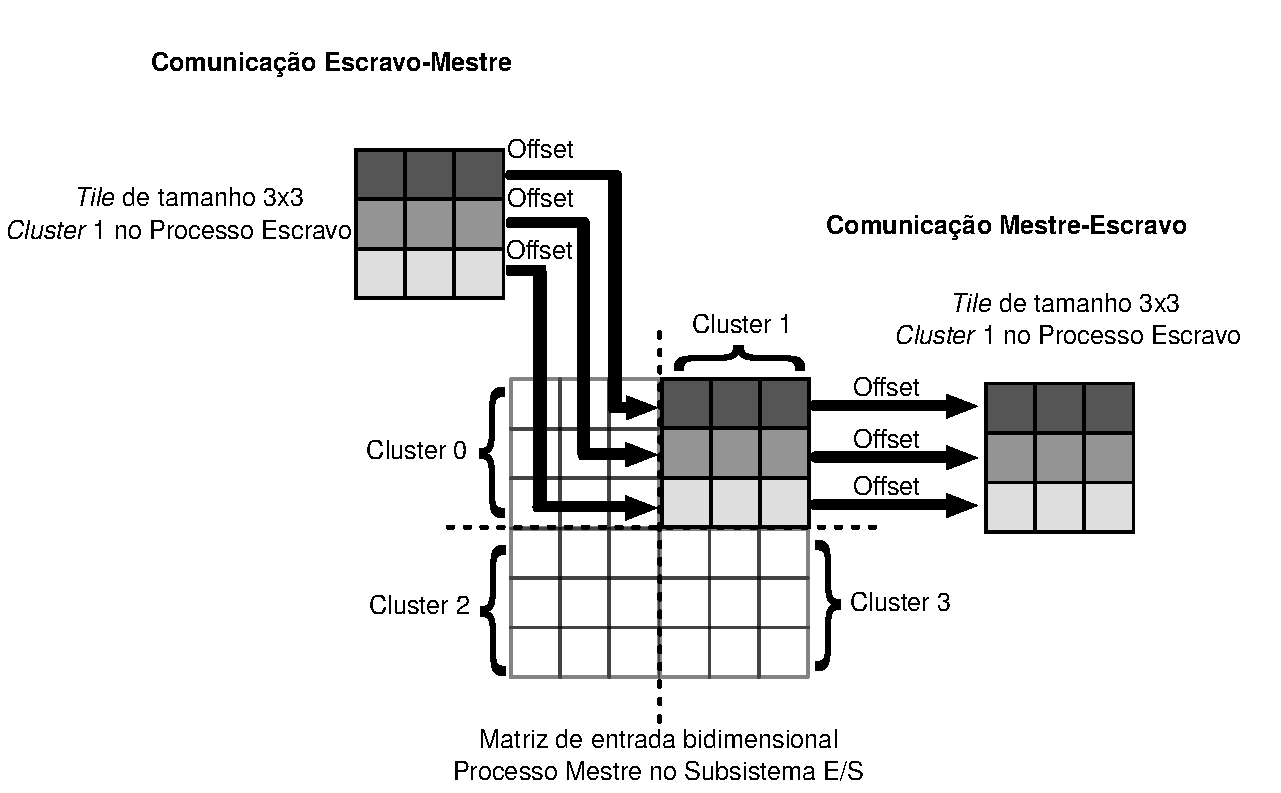
\includegraphics[width=0.7\textwidth]{figs/stridesImage.pdf}
	\caption{Exemplo do funcionamento do método \textit{strides} do \mppa.}
	\label{fig:strides}
\end{figure}

O escalonamento dos \textit{tiles} nos \textit{clusters} é feito de maneira
circular (\textit{round-robin}). Devido a isso, alguns \textit{clusters} podem
receber mais \textit{tiles} que outros, dependendo do número de \textit{tiles} e
\textit{clusters} usados na computação. Toda a comunicação entre o mestre e os
escravos é feita utilizando-se a \api de comunicação assíncrona oferecida pelo
processador \mppa. A comunicação com cada processo escravo é feita de forma
individual, mapeando diretamente áreas contíguas de memória de seus respectivos
\textit{tiles}. Além disso, a implementação atual permite a execução de
aplicações estêncil iterativas. Nesse caso, o escalonamento dos \textit{tiles} e
a computação dos mesmos pelos \textit{clusters} é repetida a cada iteração da
aplicação.

Cada processo escravo realiza a computação do \textit{tile} recebido no
\textit{cluster} utilizando o \textit{kernel} de computação estêncil definido
pelo usuário. A paralelização da computação dentro do \textit{cluster} é feita
com auxílio da \api OpenMP. Em cada \textit{cluster} podem ser criadas até 16
\textit{threads} (uma para cada \pe), onde cada uma é responsável por executar o
\textit{kernel} estêncil em um subconjunto de elementos dos \textit{tiles}.
Quando a computação do \textit{kernel} estêncil é finalizada, os \textit{tiles}
resultantes são enviados pelos processos escravos para o processo mestre, onde
são agrupados em um único \texttt{Array}, constituindo o resultado final da
computação estêncil em uma iteração. Tendo em vista que os \textit{tiles} são
regiões contíguas na memória, processos escravos precisam gerenciar os
\textit{offsets} de dados para escrevê-los nas posições corretas no
\texttt{Array} no processo mestre. Esse gerenciamento é efetuado pela \api do
\mppa, mais especificamente, pelo método de \textit{strides} mencionado
anteriormente. A Figura~\ref{fig:strides} ilustra esse procedimento para o caso
de um \texttt{Array2D}.

Para fornecer uma maior facilidade ao usuário, todas as tarefas complexas
relacionadas com a técnica de \textit{tiling}, comunicações \noc e adaptações
discutidas nessa seção são abstraídas, pois elas são incluídas no
\textit{back-end} do \pskel. Isso significa que aplicações desenvolvidas com o
\fw ~\pskel podem executar no \mppa sem a necessidade de modificações no código
fonte.

\section{Resultados Experimentais}
\label{sec:resultados}

Nesta seção será avaliado o desempenho e o consumo energético de aplicações
estêncil do \pskel quando executadas no \mppa e em um processador Intel Xeon
E5-2640 v4 com 10 núcleos de 2.4GHz (Broadwell). As medições de energia no \mppa
foram feitas considerando todos os \textit{clusters}, a memória, os subsistemas
de E/S e a NoC, onde foram coletadas por meio dos sensores de potência e energia
disponíveis no \mppa. Como o \mppa possui características intrínsecas do próprio
processador que garante baixa variabilidade entre as execuções, foram realizadas
somente 5 repetições de cada experimento, computando-se a média aritmética dos
valores. Todos os experimentos no \mppa consideraram 16 PEs por
\textit{cluster}. Por outro lado, as medições de consumo de energia foram feitas
no processador Intel com uso do \textit{Running Average Power Limit} (RAPL)
através da biblioteca PAPI~\cite{papi12}. Em cada experimento foram utilizadas
10 \textit{threads} (uma \textit{thread} por núcleo) sem uso de
\textit{hyperthreading}. Cada experimento foi repetido 30 vezes e a média
aritmética dos resultados foi calculada. Todos os resultados (\mppa e Intel)
apresentaram um desvio-padrão menor que 1$\%$.

É possível reduzir a quantidade de sincronizações e comunicações realizadas na
solução para o \mppa de duas maneiras: aumentando o tamanho dos \textit{tiles}
ou aumentando a quantidade de iterações sobre cada \textit{tile}. Como podemos
ver na Figura~\ref{fig:gputile}, ao aumentarmos a quantidade de iterações sobre
o \textit{tile}, precisamos aumentar o \textit{tile} lógico, formando um
\textit{tile} aumentado que será enviado para o \textit{cluster}. Desta forma,
devido às limitações de memória em cada \textit{cluster}, ao ser especificado
uma quantidade muito grande de iterações, o \textit{tile} aumentado enviado para
o escravo pode ser maior que o limite de memória de cada \textit{cluster}.
Portanto, foi fixado uma quantidade de 10 iterações sobre cada \textit{tile}.
Além disso, para os experimentos terem uma quantidade significativa de
sincronizações sobre aplicações estêncil iterativas, foi adotado 30 iterações
para cada aplicação.

\subsection{Aplicações Estêncil}

Para a realização dos experimentos foram utilizadas as seguintes aplicações estêncil:

\textbf{Fur:} modela a formação de padrões sobre a pele de
animais\footnote{{http://ccl.northwestern.edu/netlogo/models/Fur}}. Nessa
aplicação, a pele do animal é modelada por uma \textit{array} bidimensional de
células de pigmento que podem estar em um dos dois estados: colorida ou
não-colorida. As células coloridas secretam ativadores e inibidores. Ativadores
fazem uma célula central se tornar colorida; inibidores, por outro lado, fazem
uma célula central se tornar não colorida.
A diferença entre as potências dos ativadores e inibidores é responsável por
decidir a coloração da célula central, onde mais ativadores resulta em uma
célula colorida e mais inibidores resulta em uma célula não colorida. Nos casos
em que as potências dos ativadores e inibidores forem iguais, a cor da célula
permanece inalterada. A máscara contém células adjacentes à célula central e seu
tamanho é parametrizável. Neste trabalho foi utilizado $2$ vizinhos adjacentes
em cada direção.

\textbf{Jacobi:} método iterativo para resolver equações matriciais~\cite{demmel97}.
O método converge garantidamente se a matriz de entrada é restrita ou irredutívelmente dominante diagonalmente, i.e., $|u_{i,i}| > \sum_{j\neq i}{|u_{i,j}|}$, para todo $i$.
A Equação~\ref{eq:JacobiPoisson} define a computação em cada passo do método
iterativo de Jacobi para resolver a equação discreta elíptica de
Poisson~\cite{demmel97}. A solução aproximada é computada discretizando o
problema na matriz em pontos espaçados de forma equivalente por $n\times n$.\\
 \begin{equation}
 u'_{i,j} = \frac{u_{i\pm1,j} + u_{i,j\pm1} + h^2f_{i,j}}{4}
 \label{eq:JacobiPoisson}
 \end{equation}
 A cada passo, o novo valor de $u_{i,j}$ é obtido fazendo a média $h^2f_{i,j}$ dos seus vizinhos, onde $h = \frac{1}{n+1}$ e $f_{i,j} = f(ih,jh)$,
 para uma dada função $f$.

\textbf{GoL:} autômato celular que implementa o Jogo da Vida de Conway
\cite{gardner70}. O autômato é representado por um \textit{array} bidimensional,
onde cada elemento representa um indivíduo vivo ou um indivíduo morto. A máscara
do estêncil, a qual determina a interação entre o indivíduo e seus vizinhos,
considera as $8$ células vizinhas adjacentes à célula central. Dependendo dos
valores dos vizinhos, o elemento pode modificar seu estado entre vivo e
morto.\\

\begin{figure}[t]
	\centering
	\subfigure{\label{fig:furTileTime} 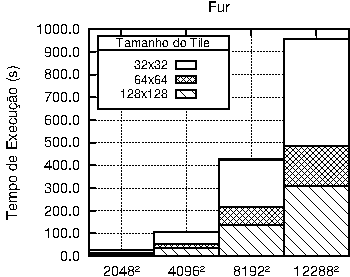
\includegraphics[width=0.27\textwidth]{figs/MPPAPlotfurTimeTiles.pdf}}
	\qquad
	\subfigure{\label{fig:golTileTime} 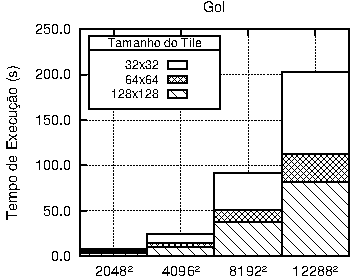
\includegraphics[width=0.27\textwidth]{figs/MPPAPlotgolTimeTiles.pdf}}
    \qquad
	\subfigure{\label{fig:jacobiTileTime} 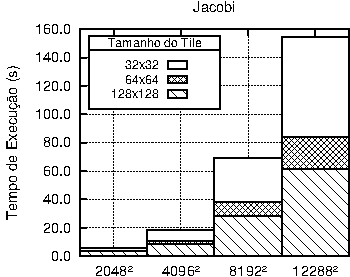
\includegraphics[width=0.27\textwidth]{figs/MPPAPlotjacobiTimeTiles.pdf}}
	\caption{Tempos de execução das aplicações para diferentes tamanhos de \textit{tile} e \texttt{Array2D} no \mppa.}
	\label{fig:timeBox}
\end{figure}

\begin{figure}[t]
	\centering
	\subfigure{\label{fig:furTileTime} 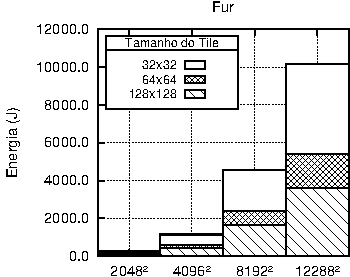
\includegraphics[width=0.27\textwidth]{figs/MPPAPlotfurEnergyTiles.pdf}}
	\qquad
	\subfigure{\label{fig:golTileTime} 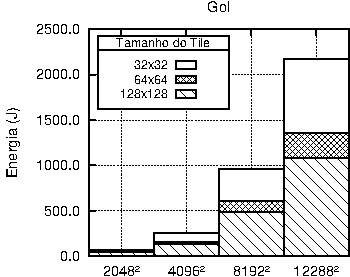
\includegraphics[width=0.27\textwidth]{figs/MPPAPlotgolEnergyTiles.pdf}}
    \qquad
	\subfigure{\label{fig:jacobiTileTime} 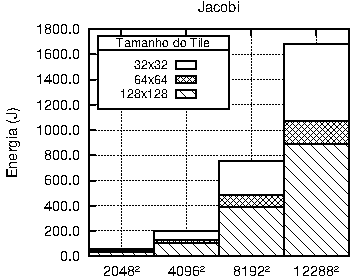
\includegraphics[width=0.27\textwidth]{figs/MPPAPlotjacobiEnergyTiles.pdf}}
	\caption{Consumo de energia das aplicações para diferentes tamanhos de \textit{tile} e \texttt{Array2D} no \mppa.}
	\label{fig:energyBox}
\end{figure}

\subsection{Impacto do Tamanho do \textit{Tile} no Desempenho do \mppa}

O primeiro experimento tem por objetivo verificar o impacto do tamanho dos
\textit{tiles} no desempenho e consumo energético das aplicações. As
Figuras~\ref{fig:timeBox} e \ref{fig:energyBox} mostram, respectivamente, os
tempos de execução e consumo de energia de três aplicações estêncil, variando-se
o tamanho do \texttt{Array2D} de entrada (de $2048^2$ até $12288^2$) e os
tamanhos do \textit{tile} (de $32^2$ até $128^2$). \textit{Arrays} de entrada
maiores que $12288^2$ e \textit{tiles} maiores que $128^2$ extrapolam às
memórias \lpddr e dos \textit{clusters}, respectivamente.

Pode-se perceber uma redução no tempo de execução à medida em que se aumenta o
tamanho do \textit{tile} (Figura~\ref{fig:timeBox}), pois há menos
sincronizações e comunicações de \textit{tiles} entre os processos mestre e
escravos. O comportamento das aplicações é similar, sendo diferenciado apenas
pela grandeza dos tempos de execução.
A Figura~\ref{fig:energyBox} apresenta um comportamento similar para o consumo
de energia, pois o tempo de execução reduz com o aumento do tamanho do
\textit{tile}, trazendo uma redução no consumo de energia.

\subsection{Análise de Escalabilidade no \mppa}

Em um segundo experimento, buscou-se verificar a escalabilidade das aplicações
no \mppa. Para isso, variou-se o número de \textit{clusters} em cada aplicação,
com \texttt{Array2D} de entrada fixo de tamanho $4096^2$ e \textit{tiles} de
tamanho $128^2$. A Figura~\ref{fig:appsTime} apresenta os tempos de execução
obtidos ao variar-se o número de \textit{clusters} utilizados na computação. A
Figura~\ref{fig:speedup}, por outro lado, apresenta o fator de aceleração
(\textit{speedup}) com relação ao tempo de execução com 1 \textit{cluster}. Em
outras palavras, o \textit{speedup} com $c$ \textit{clusters} é computado
dividindo-se o tempo de execução obtido com apenas 1 \textit{cluster} pelo tempo
de execução obtido com $c$ \textit{clusters}.

No geral, os resultados mostraram que a solução proposta para o \mppa é
escalável. Porém, pode-se notar que a aplicação \textit{Fur} apresentou uma
escalabilidade superior às demais aplicações. Esse comportamento está
diretamente relacionado com a quantidade de operações realizadas pelo
\textit{kernel} da aplicação (complexidade do \textit{kernel}). Tendo em vista a
necessidade de comunicações no \mppa, o tempo total de execução de uma aplicação
passa a ser composto pela soma do tempo de comunicação com o tempo de
computação. Para um dado \textit{tile} $t$ de tamanho fixo, o tempo necessário
para realizar comunicações de $t$ entre mestre e escravo será constante. Por
outro lado, quanto maior o número de operações (computações) feitas em $t$ pelo
\textit{kernel} da aplicação, maior será o paralelismo a ser explorado. Nesse
caso, o tempo de computação será proporcionalmente maior que o tempo de
comunicação, melhorando assim a escalabilidade obtida. Este é o caso da
aplicação \textit{Fur} cujo \textit{speedup} se aproxima do caso ideal. Em
contrapartida, aplicação \textit{Jacobi} apresentou uma escalabilidade mais
baixa que as demais, pois seu \textit{kernel} apresenta baixa complexidade.

\begin{figure}[t]
	\centering
	\subfigure[Tempo de execução.]{\label{fig:appsTime} 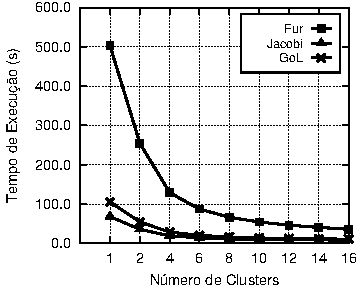
\includegraphics[width=0.32\textwidth]{figs/MPPAPlotScalability.pdf}}
	\qquad
	\subfigure[Speedup.]{\label{fig:speedup} 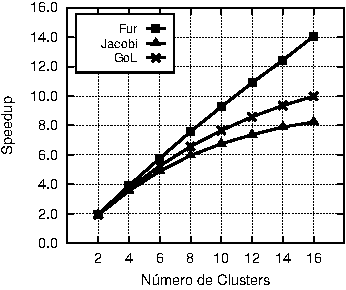
\includegraphics[width=0.31\textwidth]{figs/MPPAPlotSpeedup.pdf}}
    \caption{Resultados de tempo e \textit{speedup} das aplicações \textit{Fur}, \textit{GoL} e \textit{Jacobi}.}
    \label{fig:scalability}
\end{figure}

\subsection{Kalray \mppa vs. Intel Broadwell}

Por fim, foram efetuados experimentos comparativos entre o processador Intel
Xeon e o \mppa, como pode-se ver na Figura~\ref{fig:comparison-time}. Nesses
experimentos, utilizou-se um \texttt{Array2D} de entrada de tamanho $12288^2$ e
\textit{tiles} de tamanho $128^2$. Ao ser comparado o tempo das aplicações em
cada arquitetura, nota-se que o \mppa tem um desempenho pior, contudo ao ser
comparado o consumo de energia percebe-se um comportamento diferente: a energia
consumida pelo \mppa é menor, principalmente na aplicação \textit{Fur}. No
geral, o consumo de energia das aplicações \textit{Fur}, \textit{GoL} e
\textit{Jacobi} no \mppa foi aproximadamente $1.45$x, $1.38$x e $1.27$x menor
que no Intel Xeon, respectivamente. Por outro lado, o tempo de execução dessas
aplicações obtido no \mppa foi  $3.30$x, $2.83$x e $2.69$x maior que no Intel
Xeon, respectivamente.

%\begin{figure}[t]
%	\centering
%	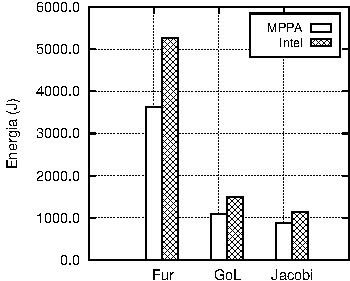
\includegraphics[width=0.4\columnwidth]{figs/ComparisonEnergyTiles10.pdf}\\
%	\caption{Comparação do consumo de energia das aplicações \textit{Fur}, Gol e Jacobi.}
%	\label{fig:comp-energy}
%\end{figure}
\begin{figure}[t]
	\centering
	\subfigure[fig:comparisonTime][Tempo de execução.]{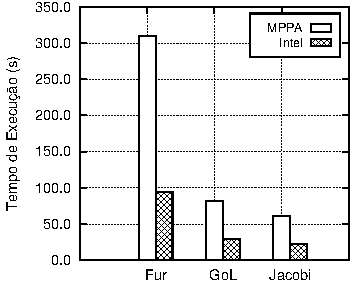
\includegraphics[width=0.32\columnwidth]{figs/ComparisonTimeTiles10.pdf}}
    \qquad
    \subfigure[fig:comparisonEnergy][Consumo de Energia.]{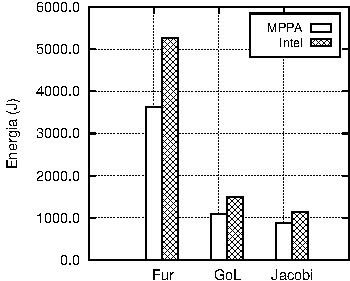
\includegraphics[width=0.31\textwidth]{figs/ComparisonEnergyTiles10.pdf}}
	\caption{Comparação do tempo de execução e consumo de energia das aplicações \textit{Fur}, \textit{GoL} e \textit{Jacobi} em relação a arquitetura.}
	\label{fig:comparison-time}
\end{figure}

\section{Conclusão}
\label{sec:conclusao}

Neste artigo foi proposta uma adaptação de um \textit{framework} para
desenvolvimento de aplicações estêncil iterativas, denominado \pskel, para
processador \mppa. A solução proposta permite esconder detalhes de baixo nível
do \mppa, simplificando significativamente o desenvolvimento de aplicações
estêncil nesse processador. Os resultados mostraram que a solução proposta
apresenta boa escalabilidade. Além disso, foi observado uma redução
significativa no tempo de execução e no consumo de energia das aplicações no
\mppa ao se utilizar a técnica de \textit{tiling} trapezoidal. Isso se deve,
principalmente, à redução do sobrecusto de comunicações e sincronizações de
\textit{tiles}.

A aplicação \textit{Fur} apresentou os melhores resultados de escalabilidade
dentre as 3 aplicações estudas, obtendo um \textit{speedup} de $14$x em relação
à execução com apenas um \textit{cluster}. Analisando experimentos executados sobre a
adaptação pôde-se perceber uma relação entre a quantidade de computação
realizada pelo \textit{kernel} da aplicação e o \textit{speedup} obtido. Por
fim, experimentos comparativos entre o \mppa e o processador Intel Broadwell
mostraram que a solução proposta para o \mppa apresenta uma eficiência
energética superior apesar de um tempo de execução superior.

Como trabalhos futuros, pretende-se estudar formas de reduzir ainda mais os
sobrecustos de comunicação através do uso de técnicas de \textit{sofware
    prefetching}. Além disso, pretende-se realizar experimentos com outros
\textit{benchmarks} e aplicações que utilizam estruturas tridimensionais. Por
fim, pretende-se realizar comparações de desempenho e consumo de energia com
outros processadores embarcados.


\bibliographystyle{sbc}
\bibliography{bibliography}

\end{document}
